%% Copyright (C) 2014 by Pascal Richter, Elena Botoeva, Richard Barnard, and Dirk Surmann
%% 
%% This file may be distributed and/or modified under the
%% conditions of the LaTeX Project Public License, either
%% version 2.0 of this license or (at your option) any later
%% version. The latest version of this license is in:
%% 
%% http://www.latex-project.org/lppl.txt
%% 
%% and version 2.0 or later is part of all distributions of
%% LaTeX version 2013/12/01 or later.
%% 

\documentclass[]{tikzposter} %Options for format can be included here

\usepackage{epsfig}
\usepackage{amsmath}
\usepackage{amssymb}
\usepackage{multicol}

\def\cparam{\mathbf{c}}
\def\R{\mathbb{R}}
\def\N{\mathbb{N}}
\def\Z{\mathbb{Z}}
\def\Q{\mathbb{Q}}
\def\C{\mathbb{C}}
\def\P{\mathbb{P}}
\def\E{\mathbb{E}}
\def\c#1{\mathcal{#1}}
\def\r#1{\text{#1}}
\def\h#1{\widehat{#1}}
\def\b#1{\mathbb{#1}}
\def\t#1{\widetilde{#1}}
\def\on{\mathrm{On}}
\def\1{\mathbbold{1}}
\def\eps{\varepsilon}
\def\diff{\backslash}
\def\d{\mathrm{d}}
\def\pd{\partial}

\def\D{\mathbb{D}}

 % Title, Author, Institute
\title{Connecting distant points via random blobs}
\author{Frankie Higgs, \texttt{fh350@bath.ac.uk}}
\institute{\Large Department of Mathematical Sciences, University of Bath\\\LARGE Based on joint work with Mathew Penrose}
\titlegraphic{
\includegraphics[scale=2.5]{images/uob-logo-grey-transparent}}

 %Choose Layout
\usetheme{Simple}

\settitle{
% To do: fix the hideous colour scheme
\centering
\vspace{30pt}
\vbox{
	\resizebox{\linewidth-100pt}{!}{\bfseries \@title}
	\vspace{20pt}
	\begin{minipage}[c]{0.5\linewidth}
		\centering
		\huge
		\@author
		
		\vspace{15pt}
		%\Large
		\@institute
	\end{minipage}
	\begin{minipage}[c]{0.4\linewidth}
		\centering
		\@titlegraphic
	\end{minipage}
	\vspace{-80pt}
}	
}

\begin{document}

 % Title block with title, author, logo, etc.
\maketitle

%\block{Abstract}{
%% A bit too long!
%% Do we even need an abstract at all?
%The \emph{random blob} model, or the Boolean model, places balls of radius $r$ centred at the points
%of a homogeneous Poisson point process $\mathcal{P}$
%in a set $A$
%with an intensity $\mu$.
%It is closely related to the random geometric graph,
%in which two points of $\mathcal{P}$
%are joined with an edge if the distance between them
%is less than $2r$.
%If the relationship between the number of balls and the radii
%is such that the average degree of a point,
%which is proportional to $\mu r^d$,
%converges to a constant
%then the model can be thought of as a form of percolation.
%
%Indeed, if $A = \mathbb{R}^d$ or a half-space and $r=1$,
%the random blob model is often called \emph{continuum percolation},
%parameterised by the intensity.
%Many well-known properties of discrete percolation are known
%to also hold for continuum percolation,
%such as existence of a non-trivial critical intensity
%and the existence of a unique unbounded component.
%
%We will discuss recent work
%on the two-point connection function
%for the Boolean model.
%%
%If $A$ is a bounded subset of $\mathbb{R}^d$
%with a sufficiently smooth boundary,
%then given distinct $x, y \in \partial A$,
%we prove a limit theorem for the probability
%that $x$ and $y$ are joined by a path in the Boolean model.
%In particular,
%if $\theta_A(\lambda)$ is the probability that the
%origin is contained in an unbounded component
%in continuum percolation with intensity $\lambda$ in $A$,
%then we show
%that if $\lambda r^d \to \mu$
%as $\lambda \to \infty$,
%then the probability that $x$ and $y$ lie in the same component
%converges to $\theta_{\mathbb{H}}(\mu)^2$.
%
%Our proof involves a renormalisation argument
%relating certain events for the Boolean model in $A$
%explicitly to corresponding events for continuum percolation
%in $\mathbb{H}$.
%}

\block{The ``random blob'' or Boolean model}{
	\begin{minipage}[c]{0.25\linewidth}
		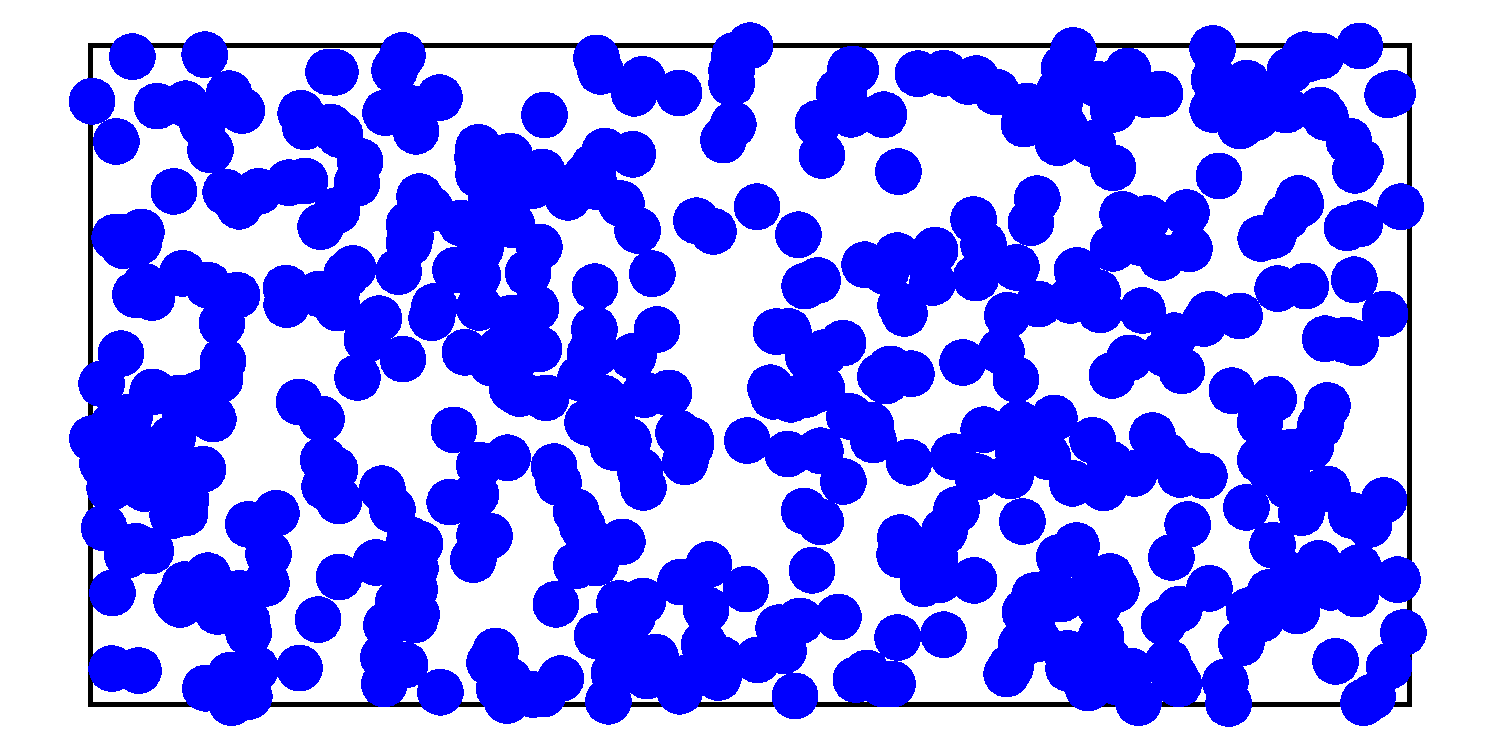
\includegraphics[width=\linewidth, trim=0 0 0 0, clip]{connection-diagram/boolean}
	\end{minipage}
	\begin{minipage}[c]{0.75\linewidth}
		Here we define the Boolean model,
		maybe give some history.
		
		The \emph{random blob} model, or the Boolean model, places balls of radius $r$ centred at the points
		of a homogeneous Poisson point process $\mathcal{P}$
		in a set $A$
		with an intensity $\mu$.
		It is closely related to the random geometric graph,
		in which two points of $\mathcal{P}$
		are joined with an edge if the distance between them
		is less than $2r$.
		If the relationship between the number of balls and the radii
		is such that the average degree of a point,
		which is proportional to $\mu r^d$,
		converges to a constant
		then the model can be thought of as a form of percolation.
	\end{minipage}
}

 \begin{columns}

 % FIRST column
\column{0.5}% Width set relative to text width

\block{Continuum percolation}{
	Let $A \subseteq \R^d$ be open, and let $\mu$ be a probability measure on $A$.
	Let $\mathcal{X} := (X_1, X_2, \dots)$ be a family of iid points distributed according to $\mu$,
	and for $n \geq 1$ let $\mathcal{X}_n := (X_1, \dots, X_n)$.
	For a given $r > 0$
	let $Z(n,r) := \bigcup_{x \in \mathcal{X}_n} B(x,r)$,
	where $B(x,r) := \{ y \in \R^d : \| x - y \| \leq r \}$.
	We call $Z(n,r)$ the \emph{Boolean model}.
	
	Suppose that $A$ is bounded,
	and take $\mu$ to be normalised Lebesgue measure.
	Without loss of generality also suppose that $A$ has Lebesgue measure 1.
}

\begin{subcolumns}
\subcolumn{0.6}
\block{Connectivity events}{
	Let $B \subseteq A$.
	Given $\mathcal{X}_n$,
	the \emph{coverage threshold}
	for $B$ is defined as
	\[
		R_n := \inf\{ r > 0 : B \subseteq Z(n,r) \}.
	\]
	If $\overline{B} \subseteq A$,
	then we can avoid boundary effects.
	The behaviour of the coverage event in this case
	has been understood since the mid 1980s
	\cite{hall85} \cite{janson86}.
	
	In this case, we have the strong law \cite{euclidean-coverage}
	\[
		\frac{n \theta_d R_n^d}{\log n} \to 1
	\]
	almost surely as $n \to \infty$,
	where $\theta_d$ is the volume of a unit ball.
	Note that $n \theta_d R_n^d$ is the total volume of the balls $\{ B(x,R_n) : x \in \mathcal{X}_n \}$.
	% whose union is $Z(n,r)$.
}
\block{}{
\centering
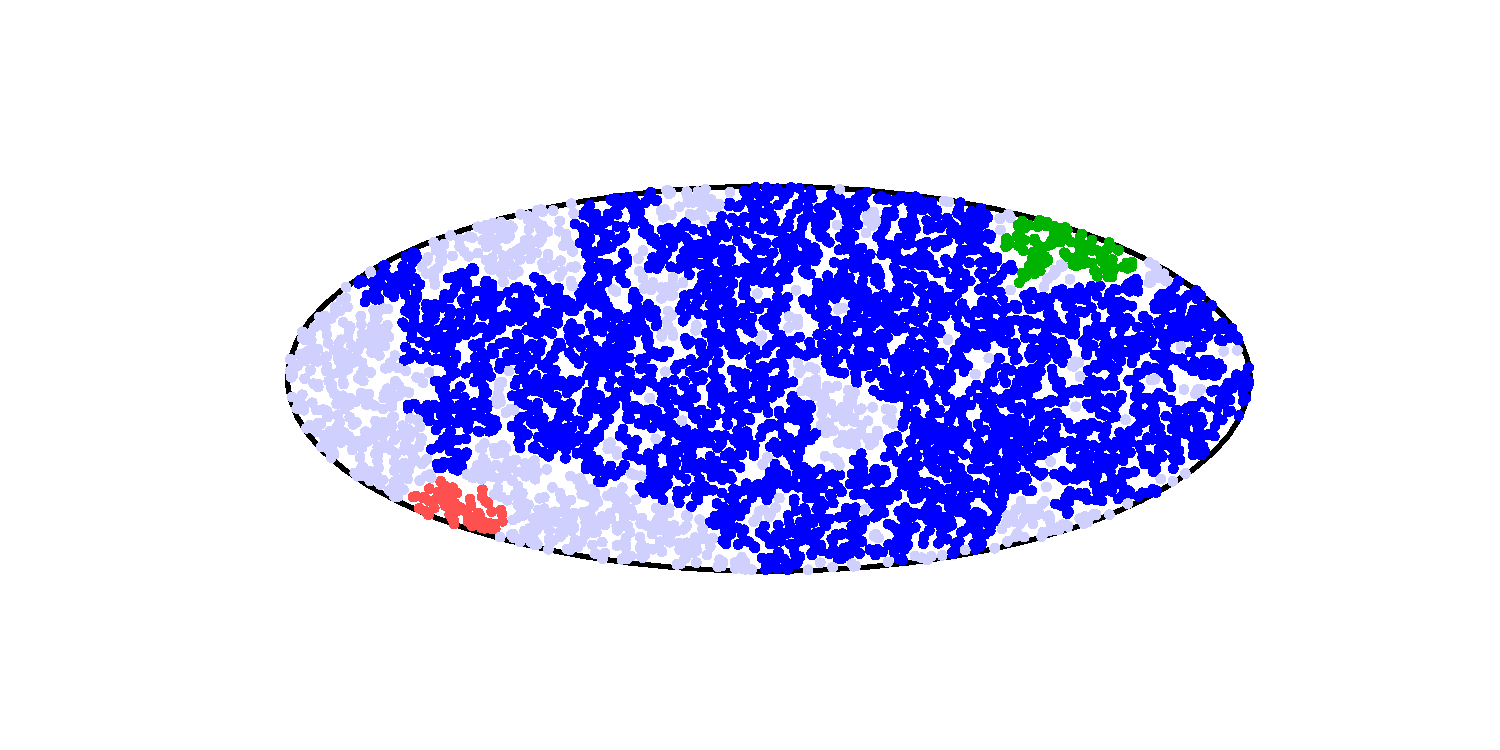
\includegraphics[width=1.0\linewidth, trim=130 80 115 85, clip]{connection-diagram/neither_percolates}
When $\lambda > \lambda_c$,
there will be a giant component.
Above,
neither $x$ nor $y$
is contained in the giant component.
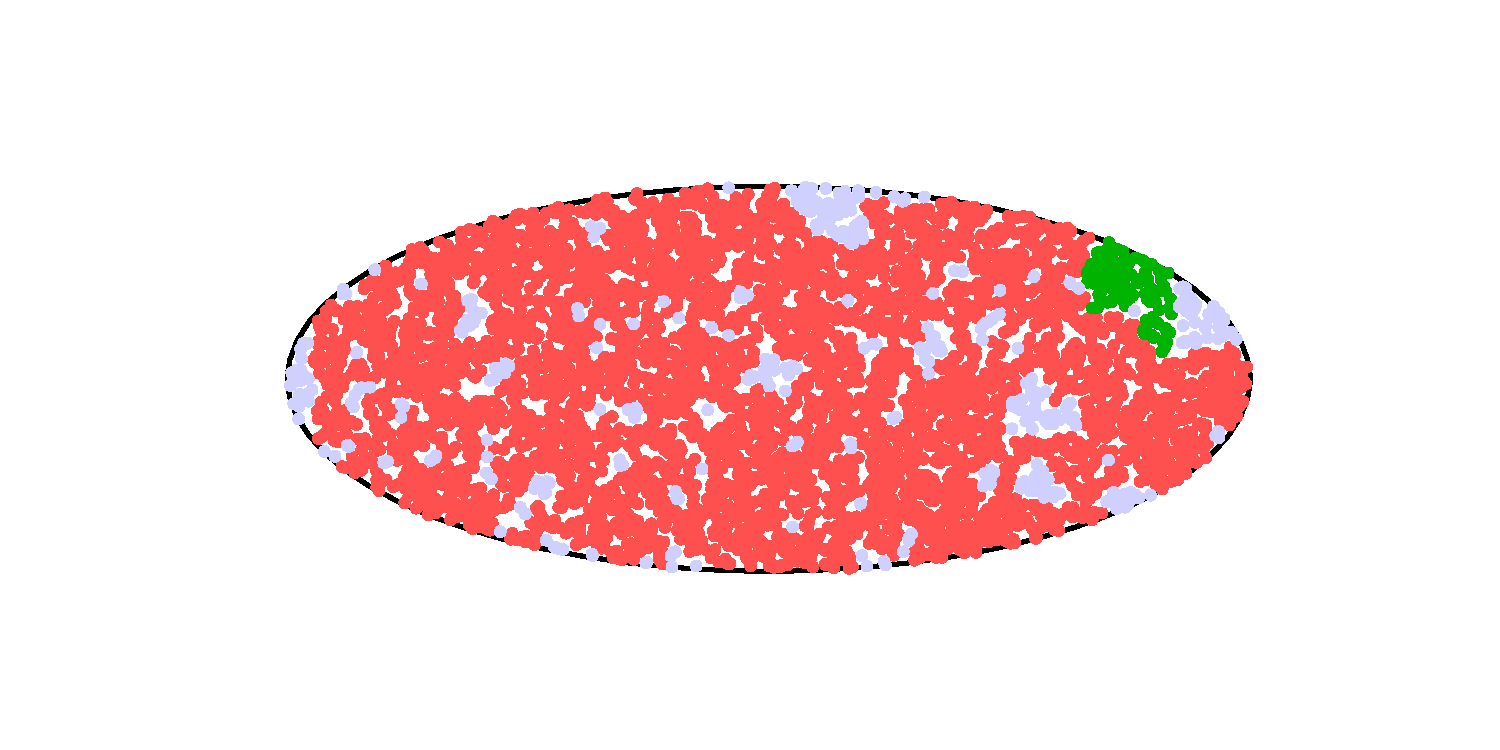
\includegraphics[width=1.0\linewidth, trim=130 80 115 50, clip]{connection-diagram/x_percolates}
$x$ is in the giant component,
but $y$ is not.
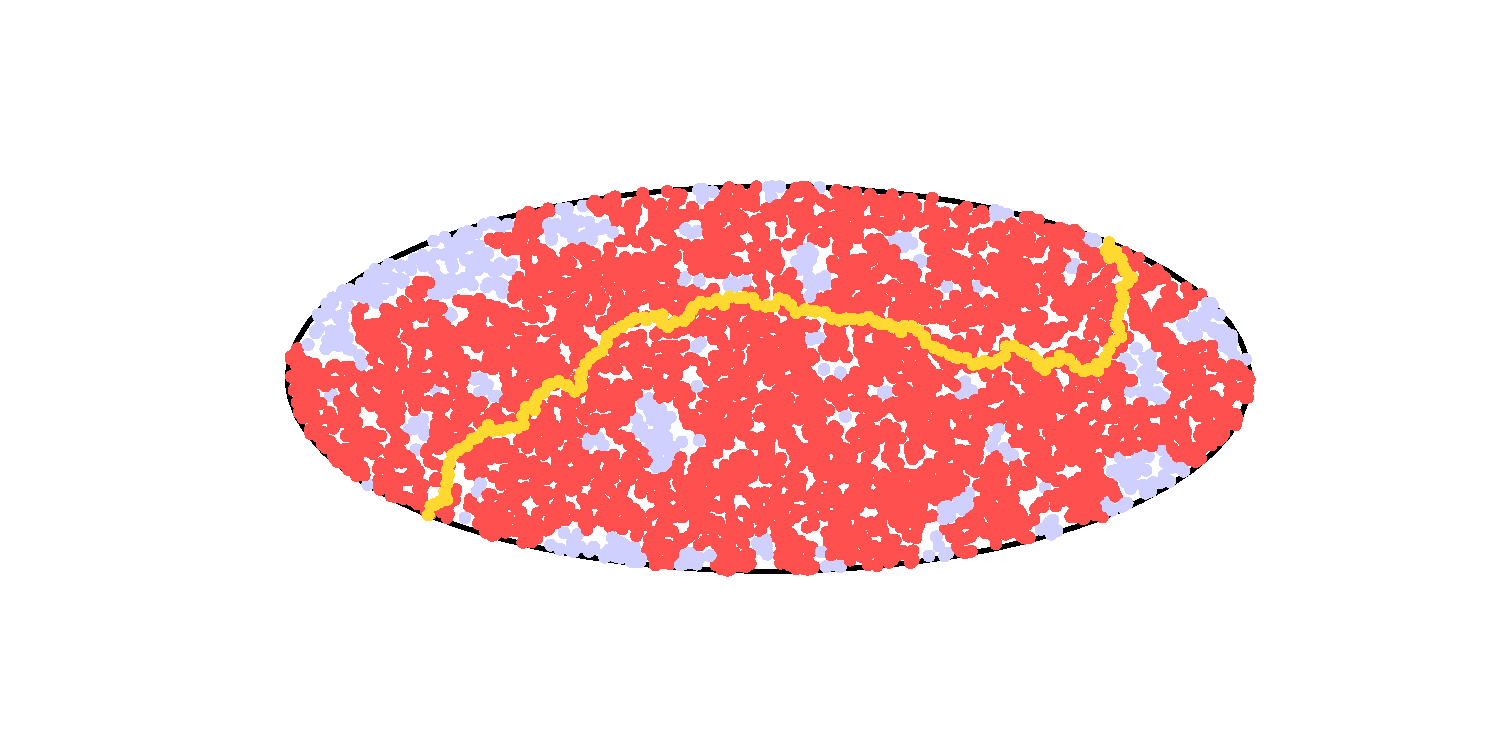
\includegraphics[width=1.0\linewidth, trim=130 80 115 50, clip]{connection-diagram/simple-path}
$x$ and $y$ are connected via the giant component.
}

\subcolumn{0.4}

\block{Does the boundary matter?}{
Yes.
}
\end{subcolumns}

\block{}{
	Similar results can be proved
	when $A$ is a Riemannian manifold with boundary.
}

 % SECOND column
\column{0.50}

\block{Renormalisation}{
	To construct long-range connections in the Boolean model,
	we define a finite grid with spacing $M r_n$ (for some large constant $M$)
	and construct a \emph{site percolation} model on this grid
	using the Boolean model.
}
\block{Events with larger blobs}
{
Some events in the $n r^d \approx \log n$ regime.

We can include some recent stuff on the ``homological thresholds.''
}

\block{}{
\vspace{-40pt}
\bibliographystyle{plain}
\begin{thebibliography}{1}

\bibitem{hall85}
Peter Hall, 1985.
\newblock Distribution of size, structure and number of vacant regions in a high-intensity mosaic.
%\newblock \textit{Z. Wahrscheinlichkeitstheorie verw Gebiete}, 1985, volume 70, pages 237--261
% I don't feel we need the full citation; author, title and year should be enough.

\bibitem{janson86}
Svante Janson, 1986.
\newblock Random coverings in several dimensions.
%\newblock \textit{Acta Mathematica}, 1986, volume 156, pages 83--118

\end{thebibliography}
}

\end{columns}



\end{document}

\endinput
%%
%% End of file `tikzposter-template.tex'.
